\documentclass[12pt]{extarticle}
\usepackage[english,ukrainian]{babel}
\usepackage[utf8]{inputenc}
\usepackage{amsmath,amssymb}
\usepackage{parskip}
\usepackage{graphicx}
\usepackage{xcolor}
\usepackage{tcolorbox}
\tcbuselibrary{skins}
\usepackage[framemethod=tikz]{mdframed}
\usepackage{chngcntr}
\usepackage{enumitem}
\usepackage{hyperref}
\usepackage{float}
\usepackage{subfig}
\usepackage{chngcntr}
\usepackage{esint}

\usepackage[top=2.5cm, left=3cm, right=3cm, bottom=4.0cm]{geometry}
\usepackage[table]{xcolor}
\newcommand{\tablespace}{\\[1.25mm]}
\newcommand\Tstrut{\rule{0pt}{2.6ex}}         
\newcommand\tstrut{\rule{0pt}{2.0ex}}         
\newcommand\Bstrut{\rule[-0.9ex]{0pt}{0pt}}   

\newcounter{exa}[chapter]
\newcounter{defi}[chapter]
\newcounter{theor}[chapter]
\newcounter{lemm}[chapter]
\counterwithin{exa}{chapter}
\counterwithin{defi}{chapter}
\counterwithin{theor}{chapter}
\counterwithin{lemm}{chapter}

\usepackage{algorithm}
\usepackage{algpseudocode}

\mdfdefinestyle{definitionStyle}{%
linecolor=blue!40!black,
outerlinewidth=1pt,%
frametitlerule=true,
frametitlefont=\sffamily\bfseries\color{white},%
frametitlerulewidth=1pt,frametitlerulecolor=blue!40!black,%
frametitlebackgroundcolor=blue!40!black,
backgroundcolor=blue!5,
innertopmargin=\topskip,
roundcorner=5pt
}

\newmdenv[style=definitionStyle]{defi}

\newenvironment{definition}[1]
  {\stepcounter{defi}%
    \addcontentsline{ldf}{figure}{#1}%
    \begin{defi}[frametitle=Означення~\thedefi: #1]}
  {\end{defi}}

\newenvironment{example}[1]
  {\stepcounter{exa}%
    \addcontentsline{ldf}{figure}{#1}%
    \begin{exa}[frametitle=Приклад~\theexa: #1]}
  {\end{exa}}

\mdfdefinestyle{exampleStyle}{%
linecolor=green!40!black,
outerlinewidth=1pt,%
frametitlerule=true,
frametitlefont=\sffamily\bfseries\color{white},%
frametitlerulewidth=1pt,frametitlerulecolor=green!40!black,%
frametitlebackgroundcolor=green!40!black,
backgroundcolor=green!5,
innertopmargin=\topskip,
roundcorner=5pt
}

\usepackage{amsmath}
\newmdenv[style=exampleStyle]{exa}

\usepackage{listings}
\usepackage{xcolor}

\definecolor{codegreen}{rgb}{0,0.6,0}
\definecolor{codegray}{rgb}{0.5,0.5,0.5}
\definecolor{codepurple}{rgb}{0.58,0,0.82}
\definecolor{backcolour}{rgb}{0.95,0.95,0.92}

\lstdefinestyle{mystyle}{
    backgroundcolor=\color{backcolour},   
    commentstyle=\color{codegreen},
    keywordstyle=\color{magenta},
    numberstyle=\tiny\color{codegray},
    stringstyle=\color{codepurple},
    basicstyle=\ttfamily\footnotesize,
    breakatwhitespace=false,         
    breaklines=true,                 
    captionpos=b,                    
    keepspaces=true,                 
    numbers=left,                    
    numbersep=5pt,                  
    showspaces=false,                
    showstringspaces=false,
    showtabs=false,                  
    tabsize=2
}

\lstset{style=mystyle}

\mdfdefinestyle{theoremStyle}{%
linecolor=yellow!40!black,
outerlinewidth=1pt,%
frametitlerule=true,
frametitlefont=\sffamily\bfseries\color{white},%
frametitlerulewidth=1pt,frametitlerulecolor=yellow!40!black,%
frametitlebackgroundcolor=yellow!40!black,
backgroundcolor=yellow!5,
innertopmargin=\topskip,
roundcorner=5pt
}

\newmdenv[style=theoremStyle]{theor}

\newenvironment{theorem}[1]
  {\stepcounter{theor}%
    \addcontentsline{ldf}{figure}{#1}%
    \begin{theor}[frametitle=Теорема~\thetheor: #1]}
  {\end{theor}}


\mdfdefinestyle{lemmaStyle}{%
linecolor=yellow!40!black,
outerlinewidth=1pt,%
frametitlerule=true,
frametitlefont=\sffamily\bfseries\color{white},%
frametitlerulewidth=1pt,frametitlerulecolor=yellow!40!black,%
frametitlebackgroundcolor=yellow!40!black,
backgroundcolor=yellow!5,
innertopmargin=\topskip,
roundcorner=5pt
}

\newmdenv[style=lemmaStyle]{lemm}

\newenvironment{lemma}[1]
  {\stepcounter{lemm}%
    \addcontentsline{ldf}{figure}{#1}%
    \begin{lemm}[frametitle=Лема~\thelemm: #1]}
  {\end{lemm}}

\title{Домашня робота \#1 з курсу ``Комплексний аналіз'' (частина друга)}
\author{Студента 3 курсу групи МП-31 Захарова Дмитра}
\date{\today}

\begin{document}

\maketitle

\section*{Завдання 1.} 

\textbf{Умова.} Розв'язати рівняння
\[
\sin z = \frac{5}{3}
\]

\textbf{Розв'язок.} Розпишемо синус як
\[
\sin z = \frac{e^{iz} - e^{-iz}}{2i}
\]

Позначимо $w := e^{iz}$, тоді маємо рівняння:
\[
\frac{w - \frac{1}{w}}{2i} = \frac{5}{3}
\]

Звідси отримуємо:
\[
\frac{w^2 - 1}{2wi} = \frac{5}{3} \to 3w^2 -10wi - 3 = 0
\]

Розв'язуємо відносно $w$:
\[
w = \frac{5i \pm \sqrt{-25 + 9}}{3} = \frac{5i \pm 4i}{3} \to w = 3i \vee w = \frac{i}{3}
\]

Отже, розглянемо випадок $w = 3i$, тобто $e^{iz}=3i$. 

В такому разі:
\[
z = \frac{1}{i}\ln 3i = -i \ln e^{\ln 3 + (\pi/2+2\pi k)i} = \frac{\pi}{2} + 2\pi k - i \ln 3, \; k \in \mathbb{Z}
\]

Аналогічно для $w=\frac{i}{3}$:
\[
z = -i \ln \frac{i}{3} = \frac{\pi}{2} + 2\pi k + i \ln 3, \; k \in \mathbb{Z}
\]

\textbf{Відповідь.} $z = \frac{\pi}{2} + 2\pi k \pm i \ln 3, \; k \in \mathbb{Z}$

\section*{Завдання 2.} 

\textbf{Умова.} Знайти $\text{Re} \cos 2i$

\textbf{Розв'язок.} Використаємо формулу:
\[
\cos z = \frac{e^{iz} + e^{-iz}}{2}
\]

Підставляємо:
\[
\cos 2i = \frac{e^{i \cdot 2i} + e^{-i \cdot 2i}}{2} = \frac{e^{2} + e^{-2}}{2} = \cosh 2
\]

В загальному випадку нескладно довести, що $\cosh r = \cos ir, r \in \mathbb{R}$.

\textbf{Відповідь.} $\cosh 2$.

\section*{Завдання 3.}

\textbf{Умова.} Знайти $\text{Im} (1-\sqrt{3}i)^{5+2i}$

\textbf{Розв'язок.} Помітимо, що
\[
1 - \sqrt{3}i = 2\left(\frac{1}{2} - \frac{\sqrt{3}}{2}i\right) = e^{\ln 2-i\frac{\pi}{3} + 2\pi k i}, \; k \in \mathbb{Z}
\]

Отже:
\[
(1-\sqrt{3}i)^{5+2i} = (e^{\ln 2-i\frac{\pi}{3}+2\pi ki})^{5+2i} = e^{(\ln 2 - i\frac{\pi}{3}+2\pi ki)(5+2i)} =: z
\]

Далі множимо вираз в експоненті:
\[
z = e^{5\ln 2 + 2i\ln 2 - \frac{5i\pi}{3} + \frac{2\pi}{3} + 10\pi ki - 4\pi k} = e^{5\ln 2 + \frac{2\pi}{3}-4\pi k}e^{2i \ln 2 - \frac{5i\pi}{3} + 10i\pi k} 
\]

Помітимо, що:
\[
\text{Im}\, e^{(2\ln 2 - 5\pi/3+10\pi k)i} = \sin\left(2\ln 2 - \frac{5\pi}{3} + 10\pi k\right) = \sin\left(2\ln 2 - \frac{5\pi}{3}\right)
\]

Отже остаточно маємо:
\[
\text{Im} (1-\sqrt{3}i)^{5+2i} = 32e^{2\pi/3-4\pi k}\sin\left(2\ln 2 - \frac{5\pi}{3}\right), \; k \in \mathbb{Z}
\]

\textbf{Відповідь.} $32e^{2\pi/3-4\pi k}\sin\left(2\ln 2 - \frac{5\pi}{3}\right), \; k \in \mathbb{Z}$.

\section*{Завдання 4.}

\textbf{Умова.} З'ясувати, в яких точках $f(z)$ є $\mathbb{C}$-диференційованою.

\begin{enumerate}
    \item $f(z)=|z|^2$
    \item $f(z)=2xy - i(x^2-y^2)$
\end{enumerate}

\textbf{Розв'язок.}

\textit{Пункт 1.} Доведемо, що ця функція диференційована лише в нулі.

Розглянемо границю:
\[
f'(z) \triangleq \lim_{\delta z \to 0} \frac{f(z+\delta z) - f(z)}{\delta z}
\]

Якщо розглянемо її в $0$:
\[
f'(0) = \lim_{\delta z \to 0} \frac{|\delta z|^2}{\delta z} = \lim_{\delta z \to 0} \frac{|\delta z|^2}{\delta z \cdot \delta z^*}\delta z^* = \lim_{\delta z \to 0} \delta z^* = 0
\]

Бачимо, що проблем немає. Проте, розглянемо $z_0 \neq 0$:
\[
f'(z_0) = \lim_{z \to z_0} \frac{|z|^2 - |z_0|^2}{z - z_0} = \lim_{z \to z_0} \frac{|z|-|z_0|}{z-z_0}(|z|+|z_0|)
\]

Доведемо, що така границя не визначена, тобто знайдемо два шляхи, вздовж яких границя різна.

Нехай ми рухаємось вздовж кола з центром в початку координат, що проходить через $z_0$ (тобто вздовж $|z|=|z_0|$, див. рис. \ref{fig:4_1}). В такому разі наша границя очевидно дорівнює $0$.

\begin{figure}[H]
    \centering
    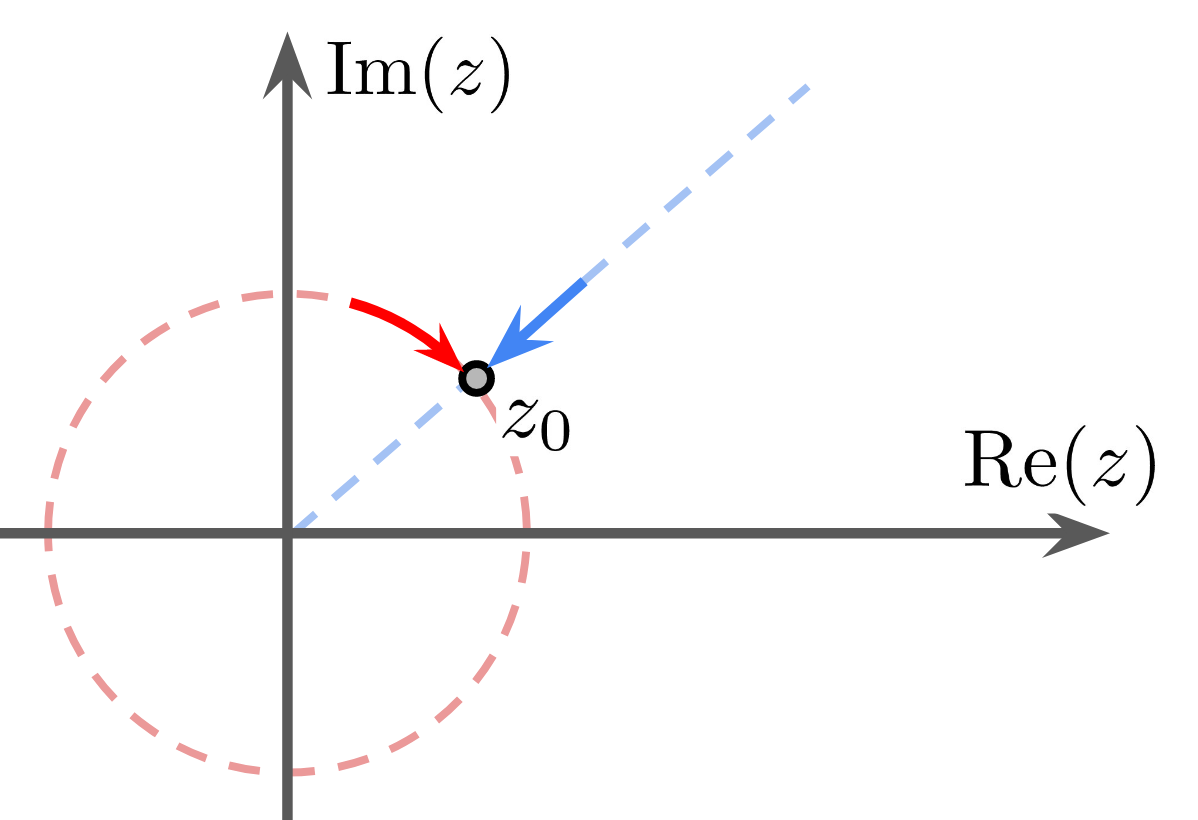
\includegraphics[width=0.7\textwidth]{images/hw_1/hw_1_4-1.png}
    \caption{\textcolor{red}{Червоним} помічена траєкторія руху вздовж $|z|=|z_0|$, а \textcolor{blue}{синім} вздовж $\mu z_0$ для $\mu \in [1,+\infty)$}
    \label{fig:4_1}
\end{figure}
\vspace{5px}

Якщо ж ми будемо рухатись вздовж променя $z=\mu z_0$ для $\mu > 1$, то:
\begin{align*}
f'(z_0) = \lim_{\mu \to 1^+} \frac{|\mu z_0| - |z_0|}{\mu z_0 - z_0} (|\mu z_0| + |z_0|) = \\
\lim_{\mu \to 1^+} \frac{|z_0|^2(|\mu| - 1)(|\mu|+1)}{z_0(\mu -1)} = \lim_{\mu \to 1^+} \frac{|z_0|^2}{z_0}(1+\mu) = 2z_0^*
\end{align*}

Ця границя в загальному випадку не дорівнює $0$, тому ми отримали дві різні границі, що означає недиференційованість у $\mathbb{C} \setminus \{0\}$.

\textit{Пункт 2.} Скористаємося умовою Коші-Рімана:

\vspace{10px}
\begin{theorem}{Умова Коші-Рімана}
    Щоб функція $f(x+iy) = \lambda(x,y) + \mu(x,y)i$ була диференційованою в $z = x_0 + iy_0$, необхідно і достатньо, аби $\lambda(x,y),\mu(x,y)$ були диференційованими в $(x_0,y_0)$ як функції дійсних змінних $x,y$ і:
    \[
    \frac{\partial \lambda}{\partial x} = \frac{\partial \mu}{\partial y}, \; \frac{\partial \lambda}{\partial y} = -\frac{\partial \mu}{\partial x}
    \]
\end{theorem}
\vspace{10px}

В нашому випадку $\lambda(x,y) = 2xy, \mu(x,y) = y^2 - x^2$. Обидві функції є диференційованими на $\mathbb{R}^2$, отже наш цікавить лише умова з частковими похідними:
\[
\frac{\partial \lambda}{\partial x} = 2y, \; \frac{\partial \mu}{\partial y} = 2y \implies \frac{\partial \lambda}{\partial x} = \frac{\partial \mu}{\partial y}
\]
\[
\frac{\partial \lambda}{\partial y} = 2x, \; \frac{\partial \mu}{\partial x} = -2x \implies \frac{\partial \lambda}{\partial y} = -\frac{\partial \mu}{\partial x}
\]

Отже, наша функція $f$ є диференційованою на всьому $\mathbb{C}$.

\textbf{Відповідь.} 1. Лише в $z = 0$. 2. На всьому $\mathbb{C}$. 

\end{document}

